% #############################################################################
% This is Chapter 1
% !TEX root = main.tex
% #############################################################################
% Change the Name of the Chapter i the following line
\fancychapter{Introduction}
\clearpage
% The following line allows to ref this chapter
\label{chap:chap001}
\noindent

The introduction section of a PhD thesis is a critical component that sets the stage for the entire document, providing a comprehensive overview of the research topic, its significance, and the specific research questions or hypotheses being addressed.
It establishes the context and rationale for the study, clearly articulating the gap in existing literature that the research aims to fill.
This section outlines the objectives of the thesis and may also preview the methodology and structure of the study, guiding the reader through what to expect in the subsequent chapters.
The introduction is pivotal in engaging the reader's interest, laying the groundwork for the argument or narrative that unfolds, and it sets the tone for the scholarly work, demonstrating the relevance and potential impact of the research within the field.

\section{Section 1}
\label{sec:chap001001}

Acronyms are abbreviated phrases or names created using the initial letters of each word in the phrase and pronounced as a single word.
They simplify longer names or phrases, making them easier to remember and quicker to say.
Acronyms are common in various fields to facilitate concise and efficient communication.
For example, ``\acs{AI}'' is an acronym for \acl{AI}.
The term can also be first used as \ac{AI} and more.

%%%%%%%%%%%%%%%%%%%%%%%%%%%%%%%%%%%%%%%%%%%%%%%%%%%
\begin{figure}[ht]
\centering
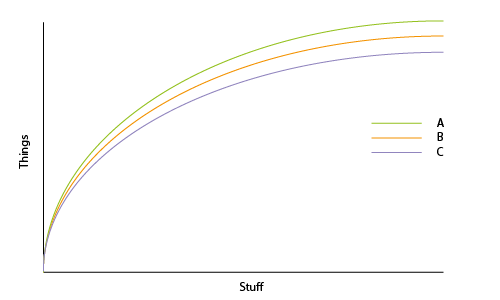
\includegraphics[width=\textwidth]{images/fig001}
\caption{This image represents an enlarged PNG derived from the preceding, smaller illustration.
Instances of figures with such inadequate quality have been observed.
It is imperative to ensure that the image maintains clarity when printed, not solely on the display screen.
Consequently, should there be any uncertainty regarding its clarity, it is recommended to perform a test print to verify its legibility.}
\label{fig:fig001}
\end{figure}
%%%%%%%%%%%%%%%%%%%%%%%%%%%%%%%%%%%%%%%%%%%%%%%%%%%

\section{Section 2}
\label{sec:chap001002}

Footnotes\footnotemark[1] are notes placed at the bottom of a page within a document or publication.
They are used to provide additional information, clarify data, cite sources, or offer explanatory comments related to specific parts of the text found in the main body.
Each footnote is typically indicated in the text by a superscript number or symbol following the relevant passage.
The reader can then refer to the corresponding number or symbol at the bottom (foot) of the page to read the additional information.
Footnotes allow authors to elaborate on specific points without interrupting the flow of the main text, making them a valuable tool for academic writing, scholarly articles, and books where detailed citations or explanations are necessary to support the content or provide further reading.

%%%%%%%%%%%%%%%%%%%%%%%%%%%%%%%%%%%%%%%%%%%%%%%%%%%
\footnotetext[1]{A footnote is a note placed at the bottom of a page in a document, providing additional information, clarification, or citations related to specific text in the main body.
It is typically marked by a superscript number or symbol in the text, directing readers to the corresponding note at the page's foot for extra details without interrupting the flow of the main content.}
%%%%%%%%%%%%%%%%%%%%%%%%%%%%%%%%%%%%%%%%%%%%%%%%%%%

LaTeX tables are structured data sets arranged in rows and columns to organize and present information clearly and concisely within a document ({\it e.g.}, Table~\ref{tab:tab001}).
LaTeX, being a powerful typesetting system, offers robust capabilities for creating complex tables.
Creating tables in LaTeX is primarily handled through the tabular environment, which allows for precise control over table layout, alignment, and formatting.

%%%%%%%%%%%%%%%%%%%%%%%%%%%%%%%%%%%%%%%%%%%%%%%%%%%
\begin{table}[htbp]
\begin{tabular*}{\textwidth}{ c @{\extracolsep{\fill}} c c @{\extracolsep{\fill}} c c @{\extracolsep{\fill}} c c }
\toprule
\\
\small
&
\multicolumn{2}{ c }{Mental Demand}
&
\multicolumn{2}{ c }{Physical Demand}
&
\multicolumn{2}{ c }{Temporal Demand}
\\
\cmidrule(lr){2-3}
\cmidrule(lr){4-5}
\cmidrule(lr){6-7}
Condition & F & Sig. & F & Sig. & F & Sig. \\
\\
\bottomrule
\\
Current & 3.392 & 0.027$\star$ & 11.99 & 0.001$\star$ & 10.51 & 0.001$\star$ \\
Assistant & 0.638 & 0.594 & 2.852 & 0.048$\star$ & 0.035 & 0.991 \\
\\
\bottomrule
\hfill
\end{tabular*}
\caption{The ANOVA factorial analysis table regarding NASA-TLX for {\it Mental Demand (MD)}, {\it Physical Demand (PD)} and {\it Temporal Demand (TD)}, where {\it F} is the variation between sample means and the variation within samples. To determine whether any of the differences between the means are statistically significant, the {\it Sig.} was used for significance. On the present study, a 20-point Likert Scale was used regarding Workload. The factorial analysis was described assuming $\alpha = 0.05$. Also, each time $p < 0.05$ it is marked with the $\star$ symbol.}
\label{tab:tab001}
\end{table}
%%%%%%%%%%%%%%%%%%%%%%%%%%%%%%%%%%%%%%%%%%%%%%%%%%%

Citations and references are integral to scholarly writing~\cite{Knuth1998}, serving to acknowledge the use of others' ideas, words, or data, and guiding readers to the original sources of information.
Citations, appearing as brief notations within the text, link to detailed bibliographic entries in the reference list at the document's end, providing full details like the author's name, publication year, and title.
This system not only attributes work to its original creators, thereby avoiding plagiarism, but also supports the verification of information and facilitates academic discourse by allowing readers to trace the research foundation upon which the document is built.
The adherence to specific citation styles ensures consistency and comprehensiveness in academic communications, reinforcing the integrity and credibility of scholarly work.